\section{Técnicas de clasificación}

\subsection{Learning from scratch}

\emph{Para ver el código para la clasificación ver archivo \archive{scratch.py} del \href{https://github.com/Griger/Intel-CervicalCancer-KaggleCompetition}{Repositorio de GitHub de la asignatura}. Además las imágenes se escalan con el código contenido en \archive{script.py}. Finalmente las predicciones de cada modelo se obtienen con el script \archive{test.py}}\\

Como primera técnica vamos a utilizar \textit{learning from scratch}. La idea básica de esta técnica es crear una red neuronal, seleccionando manualmente las capas, es decir, estableciendo tu topología, y posteriormente entrenarla. En un primer momento decidimos crear una red neuronal con una serie de capas de convolución, maxpolling, dropout, flatten y dense. Para ello creamos un modelo utilizando la clase \code{Sequencial()} de \code{Keras} (para esto nos inspiramos en el \textit{script} encontrado en un \textit{kernel} de la competición que se enlaza en la bibliografía). Una vez creado el modelo, se le añaden las distintas capas usando el método \code{add}, al que le pasamos el tipo de capa y sus parámetros. Estos parámetros varían dependiendo del tipo de capa.

\begin{itemize}
\item Para la capa de Convolución disponemos de los parámetros \textit{input\_shape}, que es el tamaño de la entrada, \textit{activation}, función de activación, el número de convoluciones a realizar y el tamaño de la matriz, esto viene de la forma (4,3,3), 4 convoluciones con una matriz 3x3 \textit{dim\_ordering}, y el orden de la dimensión de la imagen. Este último es compartido por el resto de capas. 
\item Para la capa de MaxPolling disponemos de \textit{pool\_size}, tamaño de la ventana de polling, y \textit{strides}, factor por el cual reducir la escala
\item Para la capa de Dropout contamos con \textit{rate}, cantidad de información a desechar.
\item Para la capa de Dense necesitamos \textit{activation}, función de activación, y las dimensiones de la salida.
\item La capa Flatten no requiere ningún parámetro.
\end{itemize}

Finalmente el modelo con las distintas capas se compila usando \code{compile()} que recibe como parámetros el optimizador a usar y la función de pérdida.\\

En nuestro caso, la primera red con la que se realizaron pruebas contaba con la siguiente topología:

\begin{itemize}
\item Convolución aplicando 4 convoluciones con una matriz 3x3, con activación relu e input\_shape (3,16,16).
\item MaxPooling2D con pool\_size (2, 2) y strides (2, 2).
\item Convolución aplicando 8 convoluciones con una matriz 3x3, con activación relu e input\_shape (3,16,16).
\item MaxPooling2D con pool\_size (2, 2) y strides (2, 2).
\item Dropout con rate 0.2
\item Flatten
\item Dense con dimesión 12 y activation tanh
\item Dropout con rate 0.1
\item Dense con dimesión 3 y activation softmax
\end{itemize}

Con dicha red se realizaron los primeros experimentos, con \textit{input\_shapes} de 32x32 y 256x256. Al realizarlos se obtuvieron mejores resultados con las imágenes de menor tamaño, por lo que se pensó que tal vez la red sobreaprendía con imágenes grandes. Al llegar a esta conclusión se eliminaron una serie de capas del modelo para corroborar que nuestras deducciones eran correctas. Pero el resultado fue una puntuación peor que la obtenida con la topología inicial. Debido a esto, este modelo más sencillo fue desechado para posteriores experimentos.\\

Llegados a este punto, decidimos aumentar el número de capas de nuestra red, por lo que su topología varió de la siguiente manera:

\begin{itemize}
\item Convolución aplicando 1 convolucón con una matriz 3x3 con activación relu e input\_shape (3, 256, 256)
\item MaxPooling2D con pool\_size (2, 2) y strides (2, 2)
\item Convolución aplicando 2 convoluciones con una matriz 3x3 y activation relu
\item MaxPooling2D con pool\_size (2, 2) y strides=(2, 2)
\item Convolución aplicando 4 convoluciones con una matriz 3x3 y activation relu
\item MaxPooling2D con pool\_size (2, 2) y strides (2, 2)
\item Convolución, aplicando 8 convoluciones con una matriz 3x3 y activación relu
\item MaxPooling2D con pool\_size (2, 2) y strides (2, 2).
\item Dropout con rate 0.2
\item Flatten
\item Dense con dimensión 24 y activación tanh
\item Dropout con rate 0.1
\item Dense con dimensión 12 y activación tanh
\item Dropout con rate 0.1
\item Dense con dimesión 3 y activación softmax
\end{itemize}

Con este modelo fue con el que mejores resultados se obtuvieron. En un primer momento se comprobó que este nuevo modelo mejoraba los resultados del anterior, una vez verificado procedimos a entrenarlo, pero en este caso utilizando las imágenes extra junto a las imágenes base. Esto no se realizó anteriormente ya que queríamos obtener una primera red pues no sabíamos el tiempo de cómputo que requeriría entrenar utilizando todas las imágenes. Se realizaron experimentos con un tamaño de entrada de imágenes de 32x32 y de 256x256. Como era de esperar, los resultados mejoraron a los anteriores; aunque volvimos a obtener mejores resultados con las imágenes de menor tamaño. Todos estas pruebas se realizaron con un
\textit{batch\_size} de 15, y entre 50 y 100 épocas. Viendo esta tendencia a la mejora, decidimos dar el salto a \emp{data augmentation}.\\

\subsection{Data augmentation}

\emph{Ver el archivo \archive{scratch.py} donde puede verse cómo se define el generador de nuevos ejemplos. Señalar que para la experimentación anterior se alteró este código de modo que no se hiciese ningún tipo de \textit{data augmentation}, aunque ya no se cuente con esta versión del código.}\\

Para realizar el \textit{data augmentation} se utilizó el método \code{ImageDataGenerator} del paquete \code{preprocessing.image}. Dicho método tiene una gran cantidad de parámetros que nos sirven para crear nuevas imágenes a partir de las disponibles de diversas maneras, en nuestro caso hemos utilizado los siguientes:

\begin{itemize}
\item \textit{rotation\_range} con valor 180. Básicamente establece el rango en el cual se van a realizar rotaciones aleatorias.
\item \textit{width\_shift\_range} y \textit{height\_shift\_range}, ambos con valor 0.2. Rangos para cambios aleatorios horizontes y verticales.
\item \textit{shear\_range} con valor 0.2. Para realizar transformaciones de tipo cizalla.
\item \textit{zoom\_range} con valor 0.2. Para realizar transformaciones de tipo zoom.
\item \textit{horizontal\_flip} y \textit{vertical\_flip} con valor True. Para invertir las imágenes vertical y horizontalmente.
\item \textit{fill\_mode} con valor nearest. Los puntos fuera de los límites de la entrada son rellenados dependiendo del valor elegido.
\end{itemize}

En nuestro caso se ha optado por realizar un \textit{data augmentation online}, es decir, en cada época de entrenamiento se generará un nuevo conjunto de imágenes. Para ello, una vez hemos definido el generador indicamos que queremos entrenar haciendo uso de él por medio de la función \code{fit\_generator}. También debemos modificar el valor del parámetro de \textit{steps\_per\_epoch} por el tamaño del conjunto de entrenamiento/15 (valor de \textit{batch\_size}) y multiplicarlo por un otro valor, esto se va a comentar a continuación. Con este valor podemos aumentar el número de pasos que se realizan antes de avanzar a la siguiente época, lo que significa que si aumentamos el valor, se aumenta la cantidad de datos adicionales que se procesan. Dicho esto, se realizaron pruebas con tamaños de entrada 32x32 y 256x256. Para 32x32 el valor multiplicador comentado fue de 4, mientras que para 256x256 fue 10 y posteriormente 20, ya que se obtuvo un mejor resultado usando las imágenes de tamaño 256x256 que las de 32x32, al contrario de lo que pasó anteriormente. No obstante, como analizaremos más adelante al pasar a 20 el resultado se empeoró.

\subsection{Fine tuning}

\emph{Ver los archivos \archive{fine.py} y \archive{rest.py}}\\

A continuación vamos a hablar sobre \emp{\textit{fine tuning}} y los experimentos ejecutados utilizando esta técnica. En esta ocasión se cargaron 2 redes sobre las cuales se realizó \textit{fine tuning}. Dichas redes son, \emp{ResNet50} y \emp{InceptionV3}. Si queremos realizar un entrenamiento de una manera estable y consistente debemos realizar un procedimiento denominado \textit{transfer learning} antes de aplicar el propio \textit{fine tuning}. \textit{Transfer learning} consiste básicamente en emplear las capas de convolucionales de una red convolucional como un extractor de características y a continuación entrenar un clasificador con estas características, en el caso que nos ocupa estaríamos hablando de entrenar las capass \textit{fully connected} que agregamos a estas redes. Por otro lado, \textit{fine tuning} consiste en descongelar algunas capas convolucionales inferiores y reentrenar más capas.\\

A diferencia de \textit{learning from scratch} se han realizado un menor número de pruebas, ya que el tiempo de ejecución es mayor y había que emplearlo correctamente si se querían comprobar todas las cosas que se han comentando en esta memoria. Por lo que hemos realizado dos experimentos con InceptionV3 y tres para ResNet50, ya que como se verá a continuación, ofrece mejores resultados. Cabe mencionar que ambas redes esperan las entradas en tamaño 244x244, siendo la primera vez que se trabajó con dicho tamaño, y a su vez, se usan todas las imágenes disponibles, base y extra, y \textit{data augmentation} en los experimentos. Sin mas dilación, vamos a hablar con más profundida de ambas redes.\\
 
\subsubsection{InceptionV3}

Este modelo cuenta con una serie de pesos preentrenados usando ImageNet. Lo primero que debemos hacer es crear el modelo usando \code{InceptionV3} del paquete \code{keras.applications.inception\_v3}, a dicho modelo le añadimos una capa de agrupación promedio espacial global, \textit{global spatial average pooling layer}, con \code{GlobalAveragePooling2D} del paquete \code{keras.layers}. También le agregamos una capa densa, de dimensión 3 y función de activación softmax. Una vez que disponemos del modelo configurado correctamente, se procede a entrenarlo.\\

Para ello, como hemos mencionado antes, se realiza, en primer lugar \textit{transfer learning} con un total de 10 épocas, el resto de parámetros se mantienen como en \textit{learning from scratch}, ya que fueron los que mejores resultados proporcionaron. Una vez acabado, se pasa a \textit{fine tuning}. En este caso, con un total de 50 épocas. En esta red congelamos las 174 primeras capas. En esta ocasión entrenamos la red usando como optimizador de la red un Gradiente Descendente Estocástico, \code{SGD}, con un \textit{learning rate} de 0.0001, un \textit{momentum} de 0.9 (esto nor sirve para poder converger más rápido al óptimo en caso de estar en una función con una forma de \textit{meseta} en cuyo caso el SGD convergería muy lento, así el \textit{momentum} nos permite hacer que la velocidad del gradiente se siga manteniendo en la misma dirección, siendo lo usual establecer este parámetro a 0.9 una vez el aprendizaje se ha estabilizado, cosa que conseguimos gracias al \textit{transfer learning}), y como función de pérdida, \textit{sparse\_categorical\_crossentropy} (que nos sirve para calcular el error de entropía cruzada pasándole como salida esperada la etiqueta de cada entrada en lugar de un vector de ceros y unos por cada una). Se obtuvieron buenos resultados, aunque serían superados por los proporcionados por \emp{RestNet50}

\subsubsection{ResNet50}

Este modelo, en cuanto a funcionamiento por parte del usuario, es muy similar al modelo anterior, por lo que realmente, se podría utilizar el código con el que se ha entrenado InceptionV3 para hacer lo propio con ResNet50, realizando los cambios adecuados, como es natural. Para poder usar \code{ResNet50} necesitamos el paquete \code{keras.applications.resnet50}. Al modelo, se le añaden las mismas capas que se le añadieron a InceptionV3, pero en este caso, se congelan las 162 primeras capas, ya que esta red cuenta con un menor número de ellas y se dividen en lo que podríamos denonimar "patrones", por lo que decidimos congelar todas las capas hasta el inicio del último de estos "patrones". Las épocas se mantienen iguales, 10 para \textit{transfer learning} y 50 para \textit{fine tuning}. Utilizando esta red se obtuvieron resultados muy prometedores, de los mejores obtenidos, por lo que se decidió a guardar el modelo entrenado, y volver a entrenarlo usando únicamente \textit{fine tuning} con 100 épocas, lo que nos daría un total de 150 épocas durante su entrenamiento. Para nuestra decepción, los resultados no mejoraron.\\

En la siguiente gráfica se muestra cómo fue variando el \textit{accuracy} de la clasificación sobre el conjunto de validación. Como podemos ver estas mejoras se producen pocas veces a lo largo de las 50 épocas de \textit{fine tuning} (de un cambio al siguiente este valor no se mantiene constante, simplemente no mejora) y además desde la primera época a la última donde se mejora no hay una gran diferencia, de aquí que nos plateemos como trabajo futuro emplear etapas de entrenamiento más tempranas como clasificador final, para ver si el sobreaprendizaje nos está afectando o no.

\begin{figure}[H]
  \centering
  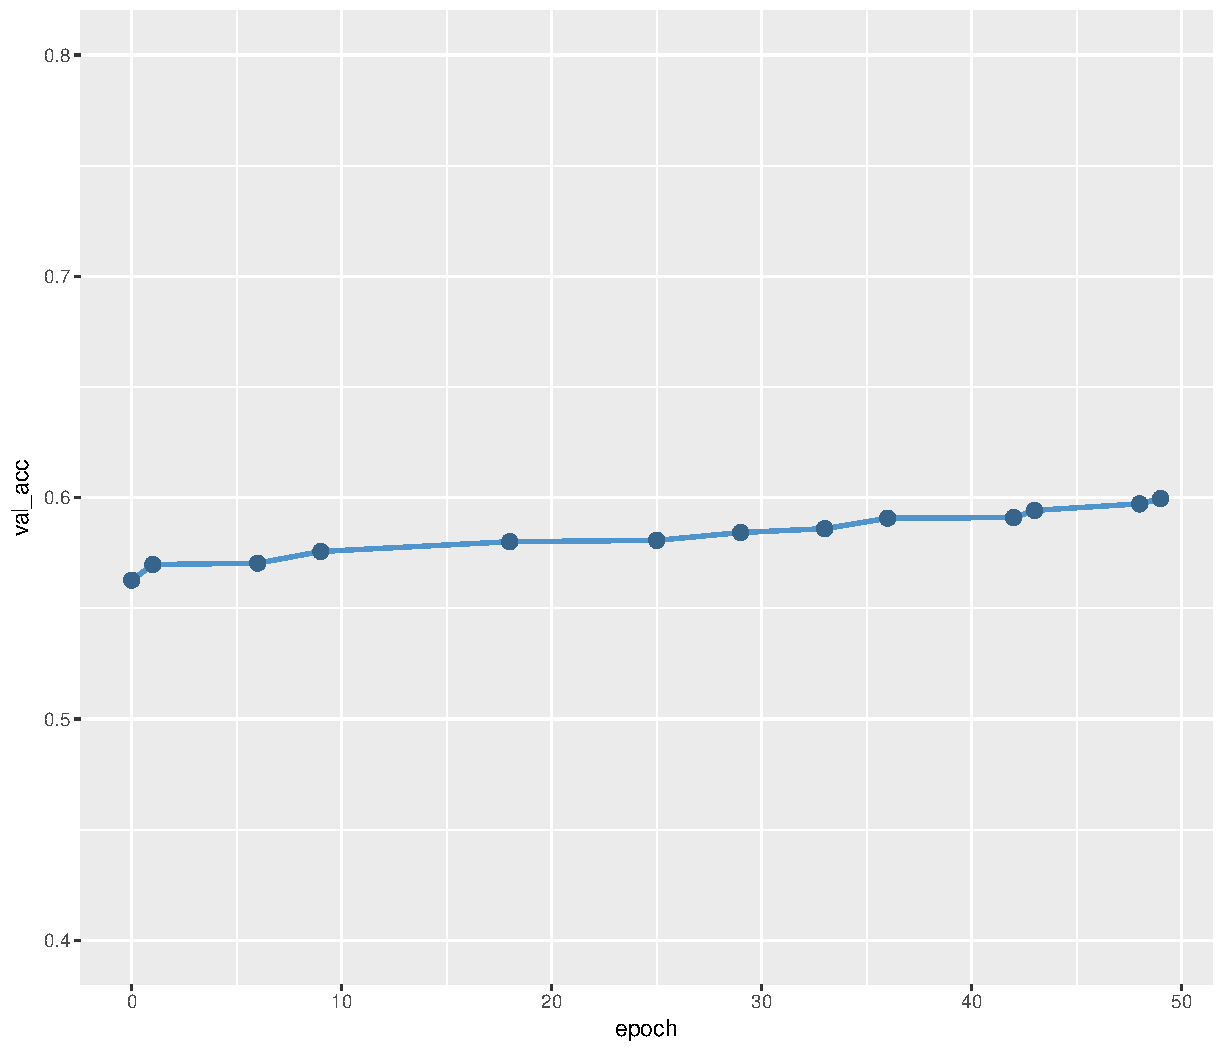
\includegraphics[scale=0.5]{img/val_acc.pdf}
  \caption{Evolución del \textit{accuracy} en el conjunto de validación.}
\end{figure}


\subsection{OVO}

\emph{Ver el archivo \archive{ovo.py} y el \archive{combine.py} para ver un ejemplo de cómo se combinarían los resultados de los tres clasificadores con los dos esquemas de agregación que se emplearon.}\\

Tras los experimentos realizados anteriormente pasamos a descomponer nuestro problema multiclase con un esquema OVO para ello entrenamos tres redes neuronales distintas, la elección de la red a entrenar la hicimos en base a los experimentos anteriores, con lo cual para cada uno de los tres problemas binarios entrenamos una ResNet 50 modificando sus capas \textit{fully connected} para que tengamos dos salidas en lugar de tres como anteriormente.\\

Se generaron, para evitar problemas con las etiquetas de cada clase, de modo que se estuviesen siempre en el conjunto {0,1} y ahora simplemente entrenamos cada una de las redes sobre cada uno de los conjunto creados, nuevamente con 10 \textit{epochs} de \textit{transfer learning} y otras 50 de \textit{fine tuning}. Una vez se han entrenado cada una de las redes pasamos al esquema de agregación de los resultados, las probabilidades, obtenidas para cada una de las clases. Señalar que para estos esquemas se ha supuesto que cada uno de las redes, para aquella clase que ignoran que existe, dan como probabilidad el valor 0.\\

El primer esquema que se nos ocurrió fue el más simple de todos, simplemente para cada clase la probabilidad asignada será \emp{la media} de la probabilidad para dicha clase asignada por cada una de las tres redes neuronales. No obstante este esquema tiene algo que no nos gusta y es que si por ejemplo tenemos las siguientes probabilidades:

\begin{table}[H]
\centering
\caption{Ejemplo de probabilidades}
\label{my-label}
\begin{tabular}{|c|c|c|c|}
\hline
Clasificador \textbackslash Clase & Tipo 1 & Tipo 2 & Tipo 3 \\ \hline
1-2                               & 1      & 0      & 0      \\ \hline
1-3                               & 1      & 0      & 0      \\ \hline
2-3                               & 0      & 0.5    & 0.5    \\ \hline
\end{tabular}
\end{table}

Entonces a esta imagen, usando como esquema de agregación la media, tenemos las siguientes probabilidades:

\begin{table}[H]
\centering
\caption{Probabilidades de la media}
\begin{tabular}{|c|c|c|}
\hline
Tipo 1 & Tipo 2 & Tipo 3 \\ \hline
0.67   & 0.17   & 0.17   \\ \hline
\end{tabular}
\end{table}

Como vemos mientras que dos clasificadores nos dan una confianza del 100\% en que la imagen es del Tipo 1, como el clasificador 2-3 da como probabilidad para esa clase el 0, puesto que no conoce el Tipo 1, y aunque ese clasificador no tiene certidumbre sobre la pertenencia de la imagen al Tipo 2 o al Tipo 3, dando probabilidad 0.5 para ambas, lo que ocurre es que la probabilidad que le damos a la imagen para el Tipo 1 es de 0.67. Esto nos parecía algo injusto y nos gustaría un esquema que tuviese en cuenta este tipo de escenarios, dando mayor peso a los dos primeros clasificadores que al que no está seguro sobre la clase a la que pertenece la imagen.\\

Por lo que acabamos de exponer decidimos probar con otro esquema, para ello leímos un artículo, en el que participa como autor el profesor Francisco Herrera y que referenciamos en la bibliografía de esta práctica, en el que se describen distintos esquemas de agregación para binarización de problemas OVO y OVA. Entre todos los esquemas expuestos nos decantamos por el llamado \emp{LVPC}, el cual se dice en el artículo que, en el caso en estar ante un problema con clasificadores binarios normalizados, es decir, clasificadores que para una clase den la probabilidad $\alpha$ y para la otra clase den su opuesto, $1 - \alpha$, entonces estamos antes un esquema establece una votación ponderada que penaliza a los clasificadores que no tienen confianza en su elección respecto a la pertenencia de la instancia a una de las dos clases que distingue.\\

Este esquema funciona como sigue, si llamamos $r_{ij}$ a la probabilidad que da el clasificador binario para las clases $i$ y $j$ para la pertenencia de una instancia a la clase $i$, y $r_{ji}$ a su análogo para la clase $j$. Entonces se calculan los siguientes términos:

\begin{center}
$P_{ij} = r_{ij} - min\lbrace r_{ij}, r_{ji} \rbrace$\\
$P_{ji} = r_{ji} - min \lbrace r_{ij}, r_{ji} \rbrace$\\
$C_{ij} = min\lbrace r_{ij}, r_{ji} \rbrace$\\
$I_{ij} = 1 - max\lbrace r_{ij}, r_{ji} \rbrace$
\end{center}

donde, como explica el artículo, $C_{ij}$ es el grado de conflicto (el grado en el que ambas clases son escogidas por el clasificador), $I_{ij}$ es el grado de ignorancia que tiene el clasificador (el grado en el que ninguna de las dos clases es escogida por el clasificador) y finalmente $P_{ij}$ y $P_{ji}$ es el grado de preferencia del clasificador hacia cada una de las dos clases. Entonces una vez que hemos calculado esto para cada instancia el esquema asigna la siguiente clase a esta instancia:

\begin{center}
$\underset{i = 1,...,m}{argmax} \underset{1 \leq j \neq i \leq m}{\sum} P_{ij} + \frac{1}{2} C_{ij} + \frac{N_i}{N_i + N_j}I_{ij}$
\end{center}

Donde $N_i$ es el número de instancias en nuestro conjunto de entrenamiento de la clase $i$. En nuestro caso, como realizamos un \textit{data augmentation online} entonces hemos supuesto que se mantienen las proporciones del conjunto de entrenamiento original, las del conjunto inicial y las adicionales para cada clase. Por otro lado como no queremos dar un resultado absoluto, es decir, dar probabilidad 1 a una clase y 0 al resto, lo que hemos hecho es en lugar de tomar el $argmax$ de las 3 sumatorias que se calculan es usar directamente el resultado de las sumatorias, dividido por 3, ya que nos encontramos con que el valor de las tres sumatorias sumaban 3 siempre, con lo que hemos dividido por tres para que sumen 1. Sin embargo los resultados obtenidos con este método para el mismo ejemplo anterior son los siguientes:

\begin{table}[H]
\centering
\caption{Probabilidades de LVPC}
\begin{tabular}{|c|c|c|}
\hline
Tipo 1 & Tipo 2 & Tipo 3 \\ \hline
0.67   & 0.19   & 0.14   \\ \hline
\end{tabular}
\end{table}

Por lo que no se soluciona el problema que queríamos evitar, seguimos teniendo la misma probabilidad para el Tipo 1, aunque sí que se penaliza al Tipo 3 en favor del Tipo 2 al haber más instancias de entrenamiento de este. Veremos adelante que además los resultados obtenidos con este método fueron peores que usando la media como esquema de agregación.

\subsection{Extracción de características con una CNN}

\emph{Ver el archivo \archive{feature.py} donde tenemos tanto el código para la extracción de características, como el código para entrenar una SVM y un modelo de GBoost.}\\

En esta ocasión el proceso fue bastante más sencillo, simplemente cargamos el modelo entrenado con la red ResNet 50, que fue el que mejor resultado nos dio de cara a la clasificación, gracias a las utilizadades de \code{Keras} que nos permiten guardar tanto la topología de la red como sus pesos, de este modo en cualquier momento se puede recuperar un modelo sin necesidad de volver a entrenarlo. Para ello cargamos el modelo con las herramientas \code{model\_from\_json} y \code{load\_weights}, y a continuación creamos un nuevo modelo a partir de este especificando que queremos como capa de salida, el parámetro \code{outputs} de la clase \code{Model}, la última de la parte convolucional de la red. Para saber qué capa escogíamos listamos los nombres de las capas de la red e identificamos el patrón de la estructura de la red y escogimos la última de convolución. Luego simplemente tuvimos que hacer una \textit{predicción} con este modelo sobre las imágenes de \textit{train} y de \textit{test} para luego usar estas características con los algoritmos que comentamos a continuación. Señalar que por falta de recurso y de tiempo en esta ocasión no se realizó \textit{data augmentation}.\\

Pasamos ahora a hablar de los dos algoritmos de clasificación que empleamos sobre este conjunto de características, 2048 para cada imagen, \emp{SVM y GBoost} ambos usados a través de la librería \code{scikit-learn} para Python. Hay que destacar que aunque esta librería no cuenta con soporte para GPU en general hemos quedado muy sorprendidos y satisfechos con el rendimiento de la implementación de estos algoritmos y la comodidad de uso que tiene toda su funcionalidad, además de la excelente documentación.

\subsubsection{SVM}

Para hacer esto creamos un modelo de predicción de tipo SVM con la función \code{SVC} de la librería \code{scikit-learn}, eligiendo que el esquema que queremos que siga para la clasificación es de tipo OVO y especificando que queremos poder obtener las probabilidades con las que ha clasificado cada una de las instancias que queremos. A continuación, y a fin de mejorar la predicción obtenida hemos creado un grid de parámetros, que se especifica usando simplemente una estructura de tipo diccionario de Python, en este grid especificamos los siguiente parámetros con los que probar:

\begin{itemize}
\item El kernel, es decir, el tipo de funciones que se usan para \textit{separar} las instancias, podrá ser o de tipo polinomial o funciones de base radial.
\item El parámetro de error C que nos indica si queremos que el hiperplano se ajuste más a los punto de \textit{training}, es decir, queremos que no se comentan muchos errores de clasificación en el train, cuando le damos a C un valor alto o si queremos un hiperplano con más margen pero que por contra cometa más errores, con una valor de C alto. En nuestro caso probamos con los valores 1 y 10.
\item La tolerancia para el criterio de parada puede ser o 0.1 o 0.001.
\end{itemize}

Entonces una vez que especificamos este grid empleamos la función \code{GridSearchCV} que buscará la mejor combinación de parámetros posible haciendo uso de un procedimiento de validación cruzada, incluso se nos da la opción de lanzar varios procesos en paralelo con distintas combinaciones de parámetros de modo que se reduzca el tiempo de cómputo. Tras este proceso por el que se seleccionan como kernel las funciones de base radial, como tolerancia el valor 0.1 y se usa como parámetro de error 10, es decir, se ajustan las funciones de base radial a los datos de entrenamiento, pasamos a entrenar el modelo con la función \code{fit} y a obtener las probabilidades de predicción sobre el conjunto de test con la función \code{predict\_proba}.

\subsubsection{GBoost}

El proceso para GBoost es muy similar sólo que ahora hacemos uso de la clase \code{GradientBoostingClassifier} y el grid de parámetros que configuramos es el siguiente:

\begin{itemize}
\item El número de árboles de regresión puede ser 50, 100 o 200.
\item Las profundidad máxima de los árboles puede ser 3 o 5.
\item La tasa de aprendizaje podrá tomar los valores 0.001, 0.1 o 1.
\end{itemize}

Tras el proceso descrito con anterioridad se llega a que el mejor conjunto de parámetros es tener 200 árboles con una profundidad máxima de 5 y empleando una tasa de aprendizaje de 0.1. Nuevamente obtenemos las probabilidades con estos parámetros.

\subsection{Extracción de características con técnicas convencionales}

\emph{Ver los archivos \archive{featureHOG.py} y \archive{featureORB.py}}

\subsubsection{HOG}

Para la extracción de características nosotros tratamos de poner en práctica dos enfoques por así decirlo, una extracción de características basada en descriptores de distintos \textit{keypoints} localizados en la escena. Este enfoque presenta una dificultad añadida de la que hablaremos en la sección correspondiente. Y por otro lado extraer una serie de características con un algoritmo que no busca \textit{keypoints} en la imagen si no que siempre extrae el mismo número de características para todas las imágenes que le pasemos.\\

En nuestro caso nos decantamos por el descriptor de características llamado \emp{Histogram of Oriented Gradients} (\textbf{HOG}) el cual es un descriptor usado en muchas ocasiones para la detección de objetos en imágenes. Este descriptor se basa en que la apariencia local de un objeto se puede describir por medio de la distribución de gradientes de intensidad.\\

Entonces la imagen (\emp{que hemos pasado a escala de grises}) se divide en varias celdas y para los píxeles dentro de esa región se obtiene un histograma de direcciones de los gradientes, siendo así la descripción de la imagen la unión de los histogramas de las distintas regiones. Además para aumentar la precisión de la descripción las celdas se agrupan en bloques, estos bloques nos sirven para medir la intensidad en un área mayor y así poder normalizar estos histogramas en base a ella.\\

Señalar que por como está pensado este descriptor es invariante para transformaciones geométricas o fotométricas, excepto para la orientación de los objetos. Aunque se conoce que estos cambios sólo se producen en grandes regiones nosotros intentamos evitar este problema, para ello intentamos realizar un \textit{data augmentation} específico en el que se generan imágenes que simplemente se\emp{ rotan arbitrariamente y a las que se les aplica un movimiento de cizalla aleatorio}. Para ello hacemos nuevamente uso de la utilidad de \code{Keras} \code{Image Data Generator}, en esta ocasión la idea era generar imágenes y almacenarlas ya que no sabíamos como hacer esto \textit{online} como lo hicimos anteriormente para entrenar una red neuronal. El problema fue que al intentar almacenar tantas imágenes obteníamos un \textit{Memory Error} con lo que tuvimos que generar sólamente una imagen por cada uno de las imágenes de \textit{train} de las que disponíamos. El objetivo era tener más imágenes en la que se vieran los tumores con distintas orientaciones y así intentar paliar esa varianza respeco a la orientación del objeto que sufre este descriptor.\\

No obstante este no fue el único problema que se presentó, y es que con el descriptor generado con los parámetro por defecto empleando la clase \code{HOGDescriptor} de OpenCV (que la usamos a través del módulo de Python \code{cv2}) obteníamos un total de \textbf{1304100} características, que no teníamos ninguna forma lógica de reducir. Podríamos haber variado los parámetros del descriptor para aumentar el tamaño de las ventanas o el de los bloques a fin de reducir el número de características extraídas pero por tiempo no pudimos hacer esto.

\subsubsection{ORB}

La otra técnica que empleamos fue una basada en la búsqueda y descripción de \textit{keypoints} en nuestro caso nos descantamos por emplear \emp{ORB} un descriptor libre desarrollado por el equipo de OpenCV y que según dicen se puede considerar una buena alternativa a otros descriptores privativos como SIFT o SURF.  ORB es una combinación del detector de \textit{keypoints} FAST y el descriptor BRIEF. No vamos a pasar a hablar en detalle de este descriptor. Simplemente comentar que para extraer los descriptores de cada imagen hemos hecho uso de la función \code{ORB\_create} de \code{cv2}.\\

Lo que vamos a hacer en su lugar es ver de qué modo podemos trabajar con las características extraídas con este tipo de técnicas de cara a la clasificación de imágenes. El problema que tienen las técnicas que se basan en la descripción de \textit{keypoints} es que no en todas las imágenes se detecta el mismo número de \textit{keypoints} y por ende no para todas las imágenes tendríamo
s el mismo número de características, un mecanismo para \textit{normalizar} este número de características es necesario.\\

Para ello se proponen dististas técnicas como la de bolsa de palabras, muy empleada en el campo de la minería de textos. En nuestro caso se ha optado por usar el algoritmo de las \emp{k-medias} de modo que dado un k todas las imágenes obtengan el mismo número de características, para ello emplearemos la utilidad de \code{scikit-learn} \code{KMeans}, estableciendo como k 500 o 2000, según el número final de características que queramos extraer.\\

El problema que teníamos en este caso es que el cómputo del algorimto de k-medias era muy costoso con lo que nuevamente obteníamos un \textit{Memory Error} con lo que tampoco se pudo probar esta técnica. También se intentó usar un detector de \textit{manchas} con un \code{SimpleBlobDetector} de OpenCV que no pudimos llegar a probar ya que obteníamos unos fallos de ejecución que no sabíamos solucionar. Este detector hubiese sido interesante ya que nos permite detectar manchas en una imagen (que podríamos identificarlas con el tumor presente en la fotografía) filtrándolas por tamaño y forma a través de sus parámetros.\\

Finalmente señalar que habrá imágenes en las que no se detecte ningún \textit{keypoint} con lo que no tendremos ninguna información para ellas: en el caso de las imágenes de entrenamiento bastará con desecharlas de cara al entrenamiento del modelo que queramos emplear para clasificar, por otro lado para las imágenes de test tendríamos que o bien dar una probabilidad igual a cada clase (0.33 en nuestro caso) o emplear otro clasificador, como una de las redes neuronales ya entrenadas para obtener una clasificación de estas instancias.